\newpage

\chapter{Elektrické výboje}
\par Následující kapitola pojednává o možnostech elektrického výboje v našem experimentu.
\par Při přípravě elektronového svazku jsme se snažili, aby byl dostatečně energetický pro dosažení prahu detekce použitého detektoru. Proto jsme cílili na dosažení elektronového svazku o energii zhruba 80 keV. Urychlení jsme prováděli pomocí rozdílu elektrického potenciálu na měděných elektrodách použitím zdrojů kladných pólů napětí. 
\par K dosažení zamýšlené energie elektronového svazku jsme použili zdroj vysokého napětí (HV) s rozsahem až do 100 kV a dva zdroje o maximálním rozsahu 5 kV. Experiment jsme prováděli ve vakuové komoře. U průchodky do vakuové komory jsme však nebyli schopni elektrody od sebe izolovat z důvodu špatné přístupnosti, takže jak z vnitřní, tak z vnější strany vakuové komory byla vzdálenost mezi elektrodami menší než jeden centimetr. V tomto místě hrozilo, že dojde k elektrickému výboji.

\section{Teorie elektrického výboje}
\par Základním dělením elektrických výbojů je dělení na samostatné a nesamostatné \cite{kracik}. Nesamostatné výboje jsou vázány na vnější (tzv. ionizační) činidlo, bez kterého nemohou probíhat. Ionizačním činidlem mohou být například elektrony vystupující ze žhavené katody nebo ozařování výbojového prostoru rentgenovými paprsky. Pokud se výboj může udržet, i když ionizační činidlo nepůsobí, nazýváme ho samostatným. Takovými výboji jsou výboje temné, doutnavé, obloukové, jiskrové, vysokofrekvenční a koróny. Dále rozebereme doutnavé a jiskrové výboje \cite{kracik}.

\subsection{Samostatné výboje}
\par Teorie samostatného výboje vznikla z rozšíření teorie nesamostatného výboje. Teorie nesamostatných výbojů je založena na myšlence Townsendových lavin, kdy žhavená katoda produkuje stálý počet elektronů za jednotku času, které dále ionizují částice plynu mezi elektrodami a produkují se laviny. U samostatného výboje již uvažujeme dostatečně vysoké napětí mezi elektrodami, že ionizační činidlo není zapotřebí a výboj probíhá pomocí vysokého počtu ionizací nárazem.
\par Minimální napětí na elektrodách, které je potřeba ke vzniku výboje $U_z$, tj. zápalné napětí samostatného výboje, lze podle Townsenda vypočítat jako \cite{kracik}

\begin{equation} 
U_z=A \frac{pd}{\ln \Big[ B \frac{pd}{\ln \big( 1+ \frac{1}{\eta_+} \big)} \Big]} \quad \text{,}
\label{eq:paschen}
\end{equation}

kde $A=BU_i$ a $U_i$ je ionizační napětí, $B=\frac{1}{p\lambda_e}$ je počet srážek na jednotku dráhy elektronu při jednotkovém tlaku prostředí, kde $\lambda_e$ je střední volná dráha elektronu a $p$ je tlak, $d$ je vzdálenost elektrod a $\eta_+$ charakterizuje vlastnosti materiálu katody, které ovlivňují pravděpodobnost emise elektronů z katody kladnými ionty (koeficient sekundární emise elektronů). Rovnice \eqref{eq:paschen} je nazývána Paschenovým zákonem. Bylo zjištěno, že konstanty $A$ a $B$ se nemění v oblasti $E/p=450-7500$ $\frac{\text{V}}{\text{kPa} \cdot \text{cm}}$ ($E$ je elektrická intenzita) a jsou rovny $A=2737,5$ $\frac{\text{V}}{\text{kPa} \cdot \text{cm}}$ a $B=112,5$ $\frac{\text{V}}{\text{kPa} \cdot \text{cm}}$ \cite{Husain1982}.
\par Průběh zápalného napětí různých plynů je znázorněn na Obr. \ref{obr:paschen}, specálně pro vzduch na Obr. \ref{obr:paschen_air}. Zápalné napětí $U_z$ nabývá minima v \cite{kracik}

\begin{equation}
(pd)_{min}=\frac{2,781}{B} \ln \Big( 1+ \frac{1}{\eta_+} \Big) \quad \text{.}
\end{equation}


\begin{figure}[h!]
\centering
\begin{minipage}[c]{200pt}
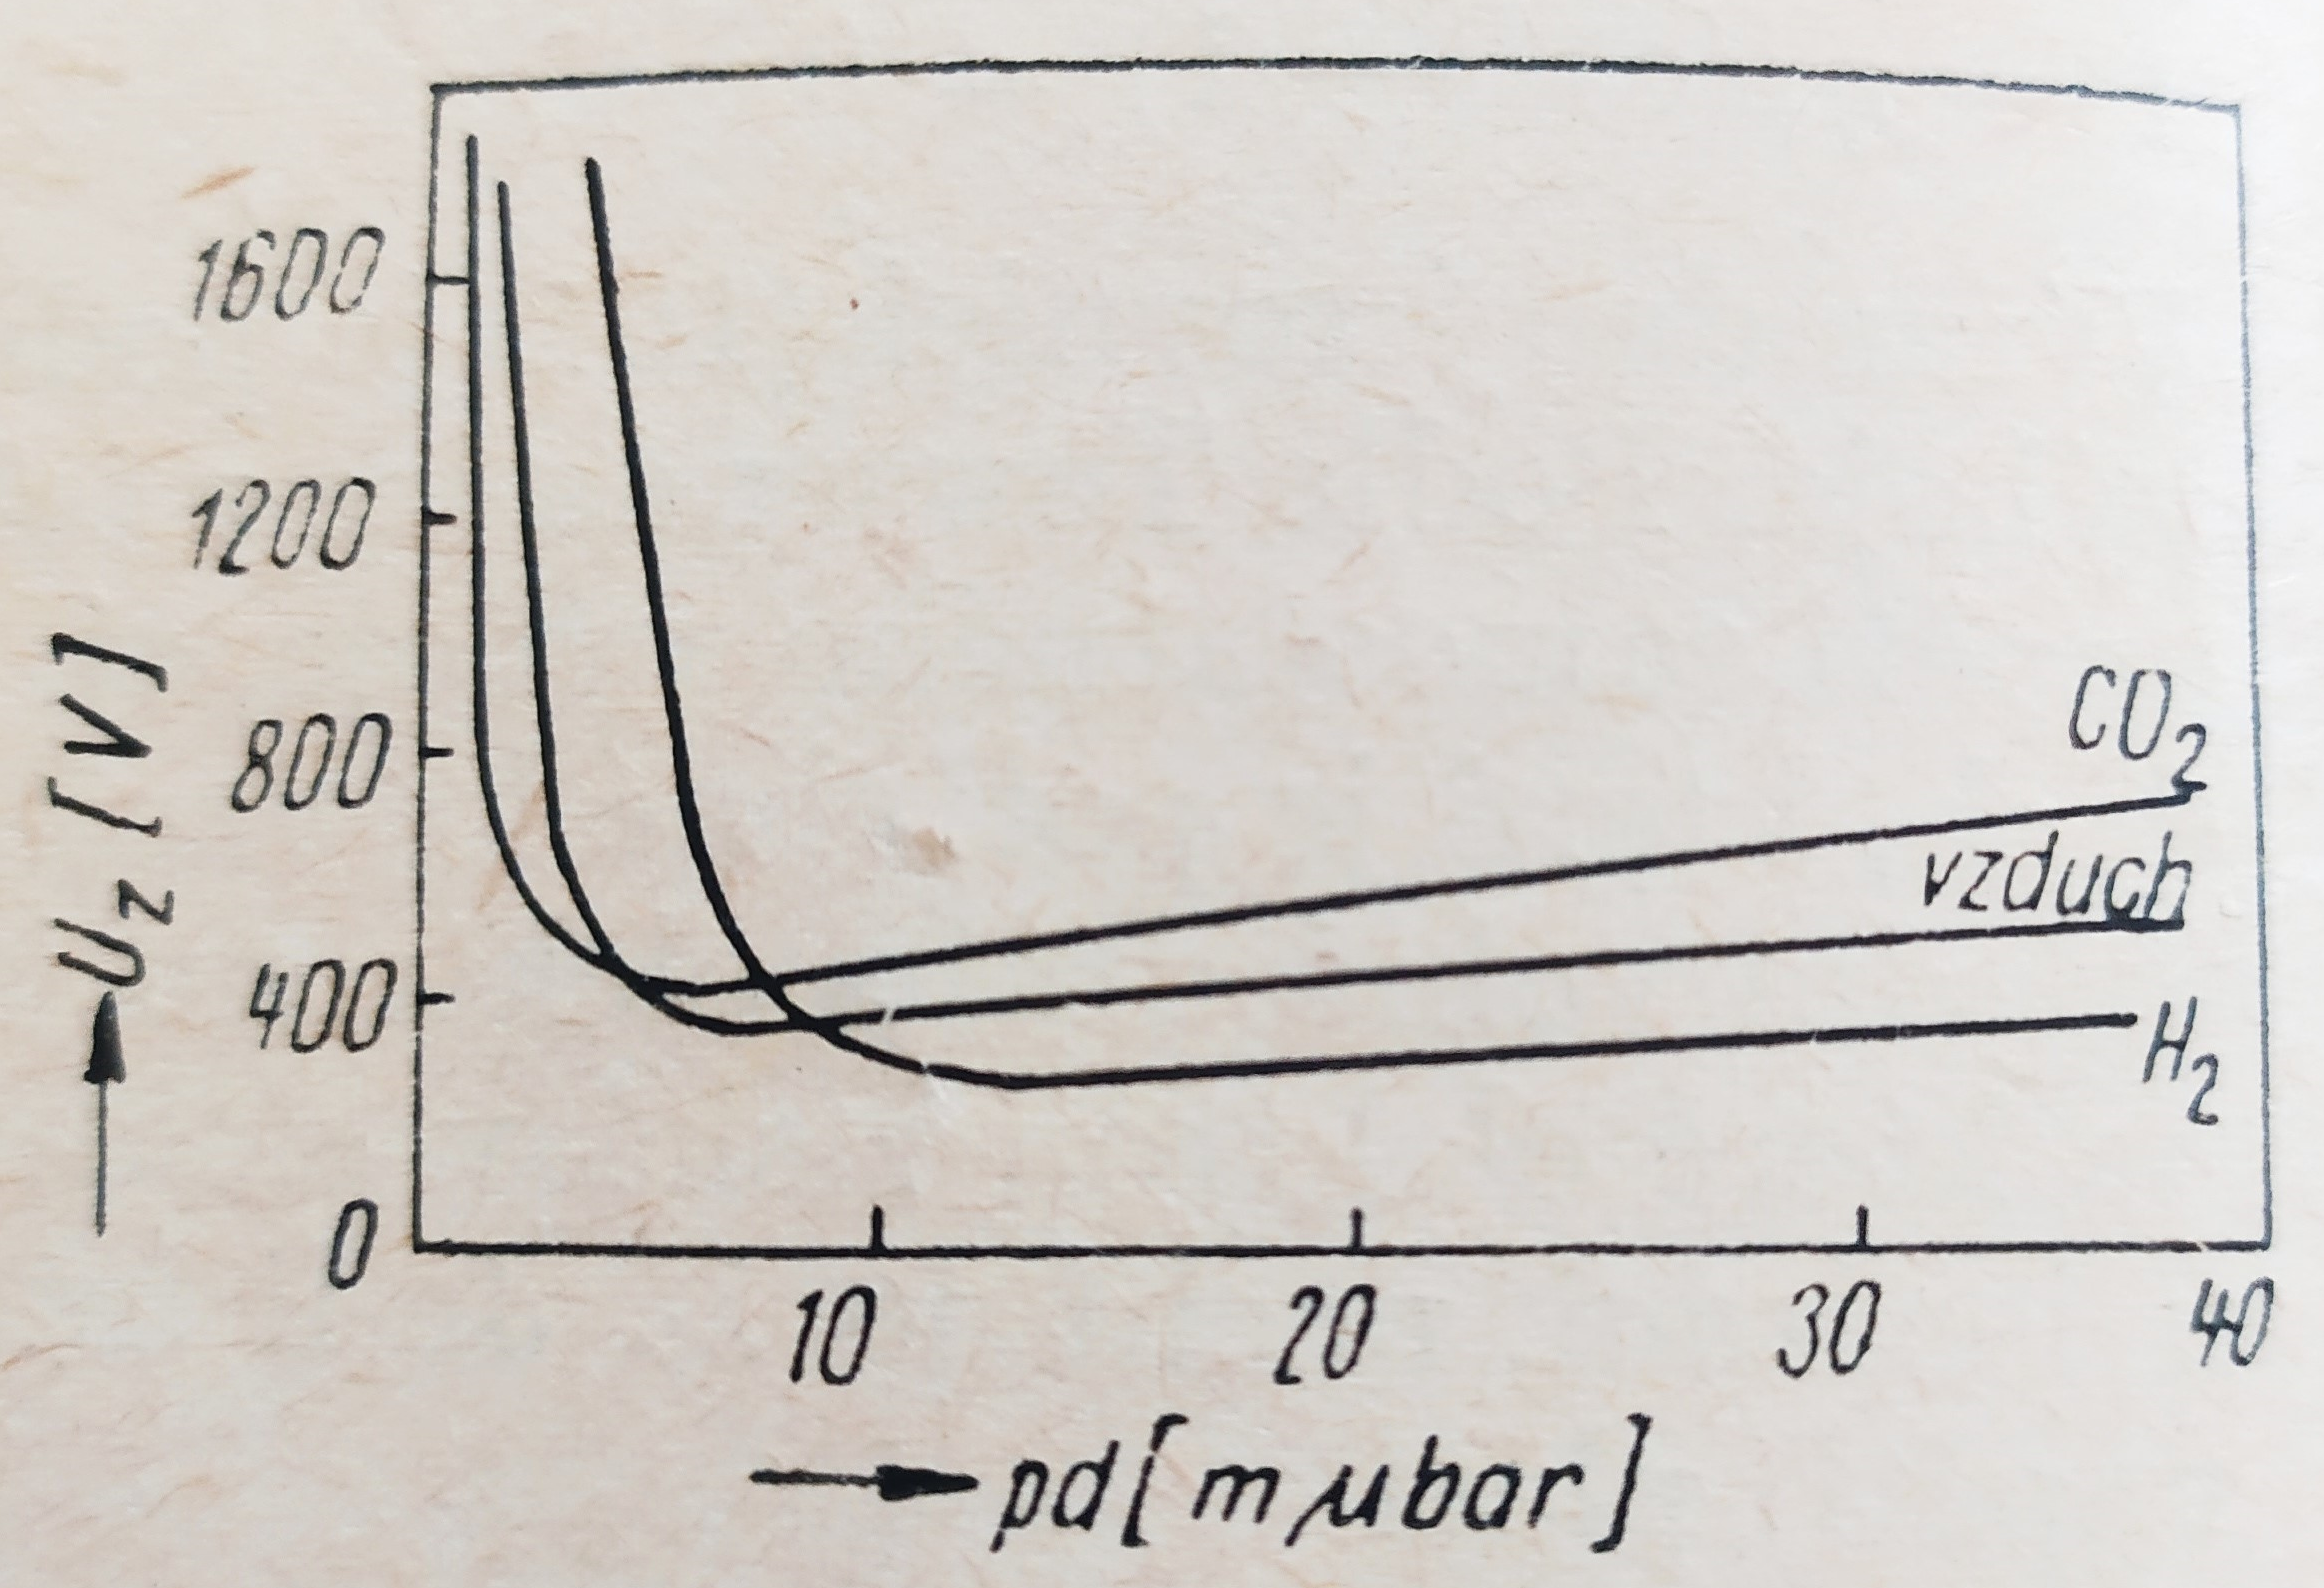
\includegraphics[width=\textwidth]{Figure/02/paschen.png}
\end{minipage}
\begin{minipage}[c]{200pt}
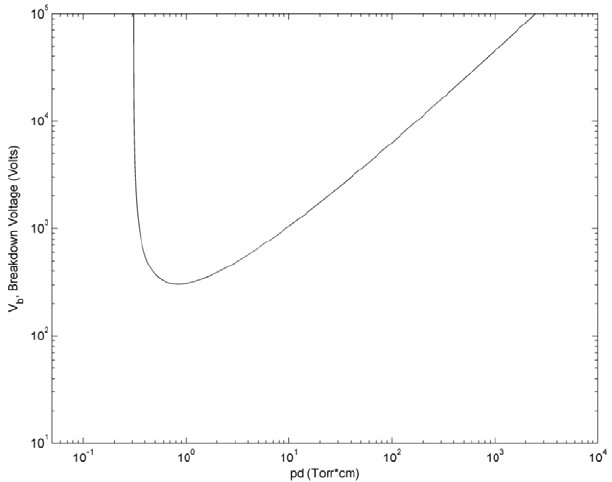
\includegraphics[width=\textwidth]{Figure/02/paschen_air.png}
\end{minipage}
\\
\begin{minipage}[c]{200pt}
\caption[Zápalné napětí různých plynů.]{Zápalné napětí různých plynů \cite{kracik}. (1~$\mu$bar = 0,1 Pa)}
\label{obr:paschen}
\end{minipage}
\begin{minipage}[c]{5pt}
\end{minipage}
\begin{minipage}[c]{200pt}
\caption[Paschenova křivka pro vzduch]{Paschenova křivka pro vzduch z roku 2011 \cite{Martins2011}. (Torr$\cdot$cm = 133 Pa$\cdot$cm)}
\label{obr:paschen_air}
\end{minipage}
\end{figure}

\subsubsection{Doutnavý výboj}
\par Přechod od nesamostatného výboje k samostatnému je doprovázeno vzrůstem proudu a světélkováním plynu. Pro doutnavý výboj jsou charakterizující světélkující oblasti především u anody, kde dochází k nejvíce srážkám elektronů s molekulami plynu \cite{kracik}. V závislosti na rozložení prostorových nábojů se průběh potenciálu mezi katodou a anodou deformuje a světélkující oblasti se nacházejí i dále od anody. Rozložení prostorových nábojů se mění i s tlakem \cite{edu-techmania}. Na Obr. \ref{obr:doutnavy} je znázorněn doutnavý výboj ve vzduchu při tlaku 100 Pa.

\subsubsection{Jiskrový výboj}
\par Jiskrový výboj je nestabilní a nestacionární forma samostatného výboje, která nevyžaduje působení ionizačního činidla \cite{kracik}. Má vzhled jasně svítících větvících se kanálů o vysoké teplotě a v plynu je doprovázen akustickými jevy. Přestože se při jiskrových výbojích uplatňuje jiný princip vzniku než při výboji lavinovém, tzv. kanálový mechanismus, platí pro ně Paschenův zákon \eqref{eq:paschen} \cite{kracik}. Jelikož se součinitel $\eta_+$ vyskytuje v Paschenově zákoně ve tvaru $\ln \ln \eta_+$, materiál katody nemá vliv na velikost $U_z$ \cite{kracik}. Zápalné napětí je nazýváno napětím průrazu a u vzduchu činí toto průrazné napětí při normání teplotě a tlaku 3 MV/m = 30 kV/cm \cite{tipler1987}.

%napočítat hodnoty napětí pro průraz s tim, že eta dáme třeba 40 podle 
%https://arxiv.org/ftp/arxiv/papers/1302/1302.2333.pdf 
%https://arxiv.org/ftp/arxiv/papers/1302/1302.2334.pdf
% dále doutnavý a jiskrový výboj a pak popis naší aparatury a co jsme pozorovali - to fialový a pak blesk, jak jsme to vyřešili (izolace nefungovala, přendání, nižší napětí)


\begin{figure}[h!]
\centering
\begin{minipage}[c]{200pt}
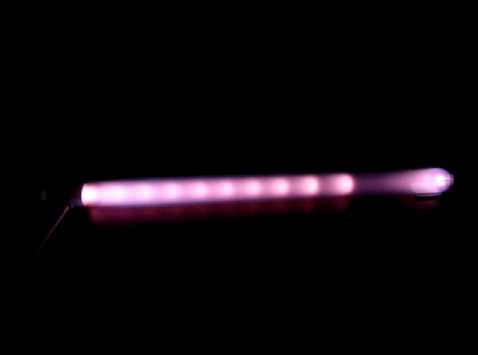
\includegraphics[width=\textwidth]{Figure/02/doutnavy.png}
\end{minipage}
\begin{minipage}[c]{200pt}
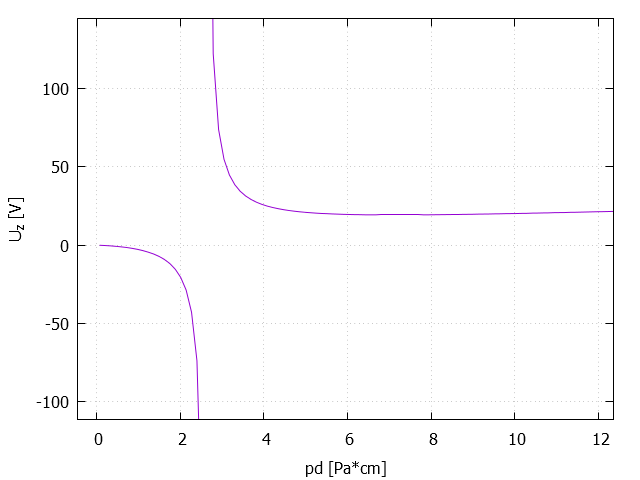
\includegraphics[width=\textwidth]{Figure/02/paschen_moje.png}
\end{minipage}
\\
\begin{minipage}[c]{200pt}
\caption[Ekvipotenciální plochy v doutnavém výboji při 100 Pa]{Ekvipotenciální plochy v doutnavém výboji při 100 Pa \cite{edu-techmania}.  }
\label{obr:doutnavy}
\end{minipage}
\begin{minipage}[c]{5pt}
\end{minipage}
\begin{minipage}[c]{200pt}
\caption[Paschenova křivka pro určité hodnoty konstant]{ Funkce f(x) je vykreslená Paschenova křivka \eqref{eq:paschen} pro hodnoty $A=2737,5$ $\frac{\text{V}}{\text{kPa} \cdot \text{cm}}$, $B=112,5$ $\frac{\text{V}}{\text{kPa} \cdot \text{cm}}$ a $\eta_+=3$.}
\label{obr:paschen_moje}
\end{minipage}
\end{figure}


\section{Přivedení vodičů k elektrodám}
\par K elektrodám, které sloužily jak pro urychlení, tak i k fokusaci elektronového svazku, jsme přiváděli jeden vodič s napětím vyšším než 20 kV a dva s napětím do 5 kV. Nejprve jsme se pokoušeli použít jedinou průchodku, u které byly všechny sousední vodiče vzdáleny méně než jeden centimetr. Podle teorie by k výboji na vzduchu mělo docházet při zhruba 20 kV/0,7 cm, což nebylo pro naše účely dostatečné a vysoké napětí jsme přiváděli samostatnou průchodkou.
% My jsme však nebyli schopni získat z vysokonapěťového zdroje více než 5 kV pravděpodobně kvůli neúmyslnému uzemnění v jiném místě. Naším cílem bylo navíc vést vodičem více než 20 kV, čímž bychom překročili dielektrickou pevnost vzduchu. Vysoké napětí jsme tedy přiváděli samostatnou průchodkou a původní průchodkou jsme vedli pouze vodiče do 5 kV. 
\par Samostatná průchodka však nebyla uzpůsobena k vedení vysokého napětí a opět byl vodič vzdálen zhruba 1 cm od uzemněné vakuové komory. I přes naši snahu nechráněné části průchodky co nejvíce izolovat vulkanickou páskou jsme při překročení napětí 30 kV na vzduchu výboje pozorovali. Vysokonapěťovou keramicky izolovanou průchodku jsme bohužel k dispozici neměli.
\par Uvnitř komory byly jednotlivé elektrody vzdáleny od sebe navzájem a od uzemněné komory také přibližně jeden centimetr. Abychom mohli použít výpočet pomocí Paschenova zákona \eqref{eq:paschen}, je potřeba, aby podíl elektrické intenzity $E$ a tlaku $p$ byl v rozmezí $E/p=450-7500$ $\frac{\text{V}}{\text{kPa} \cdot \text{cm}}$. Námi cílený tlak byl ideálně co nejmenší, abych se náš elektronový svazek nerozptyloval na molekulách vzduchu, tedy $10^{-2}-10^{-4}$ Pa. Pro napětí $U$ v řádu kilovoltů však ze vztahu $E=U/d$ dostáváme pro $d=1$ cm $E/p \sim 10^{9}$ $\frac{\text{V}}{\text{kPa} \cdot \text{cm}}$. I kdybychom se rozhodli toto omezení nerespektovat, zjistíme, že z Paschenova zákona dostaneme pro námi zamýšlené hodnoty $p=10^{-3}$ Pa a $d=1$ cm nesmyslný výsledek $U_z<0$ \footnote{Použili jsme $A=2737,5$ $\frac{\text{V}}{\text{kPa} \cdot \text{cm}}$, $B=112,5$ $\frac{\text{V}}{\text{kPa} \cdot \text{cm}}$ a $\eta_+=3$ \cite{Bozhko}. Volba jiného $\eta_+$ v rozmezí $\eta_+=2-100$ výsledek nemění.}, jelikož má závislost \eqref{eq:paschen} průběh hyberboly (Obr. \ref{obr:paschen_moje}).
%což potvrzuje neaplikovatelnost \eqref{eq:paschen}. Jelikož má závislost \eqref{eq:paschen} průběh hyberboly (Obr. \ref{obr:paschen_moje}), je chybné se domnívat, že pro námi dosahované oblasti $10^{-4}$ Pa$\cdot$cm $\sim 8\cdot 10^{-7}$ Torr$\cdot$cm by $U_z$ šlo do nekonečna (Obr. \ref{obr:paschen_air}). 
Proto jsme neexistenci výboje v komoře odhadovali pouze na základě úvahy, že při dosaženém nízkém tlaku nebude pro výboj k dispozici dostatečný počet ionizovatelných atomů a molekul.



\section{Pozorování a diskuse}
\par Při prvních zkouškách jsme dosahovali tlaku zhruba 100 Pa a při použitém napětí 3 kV jsme pozorovali fialový doutnavý výboj (Obr. \ref{obr:fialovy_vyboj}). Naše pozorování se shoduje s očekáváním z Obr. \ref{obr:doutnavy}. Současně jsme však nepozorovali žádný signál elektronů na instalovaném stínítku. Použité wolframové vlákno pravděpodobně nebylo vhodným zdrojem elektronů. 
% jako zdroje elektronů, které nám buď nedodávalo dostatečný počet elektronů, anebo jsme elektrony nebyli schopni od vlákna urychlit ke stínítku kvůli nevhodnému sestavení aparatury. 
\par Další pokusy jsme prováděli při tlaku přibližně 10$^{-2}$ Pa \footnote{Jelikož se nám ke konci semestru porouchal tlakoměr, dosažený tlak řádu 10$^{-2}$ Pa jsme odhadovali na základě alespoň třídenního čerpání vakuové komory turbomolekulární vývěvou. }. Při nich jsme již nepozorovali doutnavý výboj, ale při dosažení napětí 20 kV na urychlovací elektrodě jsme v komoře pozorovali výboje doprovázené zelenými záblesky na instalovaném fluorescenčním stínítku. Pravděpodobně se jednalo o elektrony vzniklé při výboji, které na stínítko dopadly, jelikož jsme stejné zelené světlo pozorovali na stínítku při dopadu elektronů z funkčního elektronového děla, které bylo instalováno v další fázi experimentu. Tyto výboje se v závislosti na použitém napětí pravidelně opakovaly a se zvyšujícím se napětím se časové intervaly mezi nimi zkracovaly. Pohledem do komory pomocí malého průzoru jsme bohužel nebyli schopni určit, kde k výbojům dochází. Výboje jsme pozorovali i v případě, kdy jsme zapojili pouze jednu elektrodu s nejvyšším urychlovacím napětím, domníváme se proto, že docházelo k výboji do komory v místě, kde byla vzdálenost elektrody od komory nejmenší. Při jednom výboji jsme dokonce pozorovali jasný jiskrový výboj (Obr. \ref{obr:jiskra}) bez zeleného záblesku.

\begin{figure}[h!]
\centering
\begin{minipage}[c]{200pt}
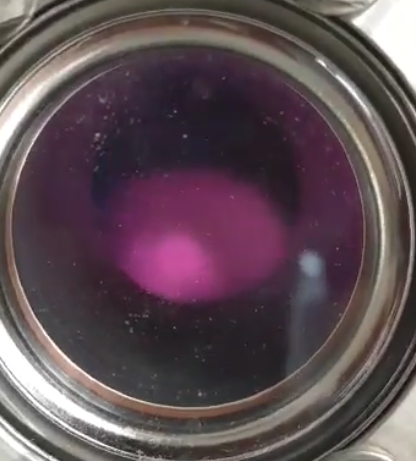
\includegraphics[width=\textwidth]{Figure/02/fialovy_vyboj.png}
\end{minipage}
\begin{minipage}[c]{200pt}
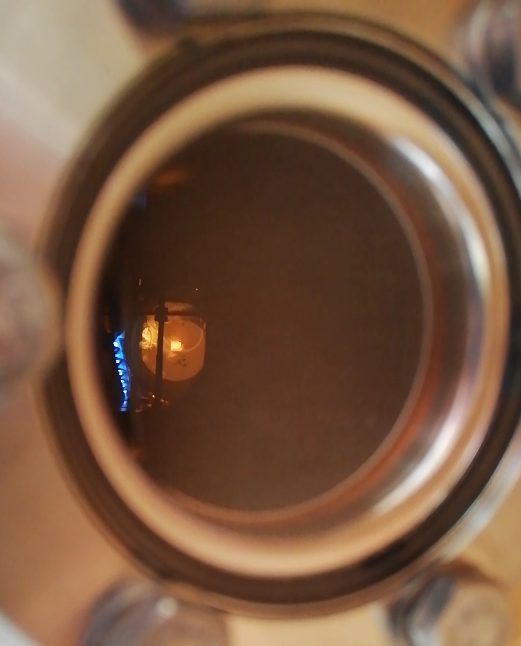
\includegraphics[width=\textwidth]{Figure/02/jiskra.png}
\end{minipage}
\\
\begin{minipage}[c]{200pt}
\caption[Pozorovaný doutnavý výboj]{Pozorovaný fialový doutnavý výboj při tlaku zhruba 100 Pa.  }
\label{obr:fialovy_vyboj}
\end{minipage}
\begin{minipage}[c]{5pt}
\end{minipage}
\begin{minipage}[c]{200pt}
\caption[Pozorovaný jiskrový výboj]{Pozorovaný jiskrový výboj při tlaku zhruba $10^{-2}$ Pa.}
\label{obr:jiskra}
\end{minipage}
\end{figure}


\par Při použití napětí vyššího než 30 kV jsme pozorovali výboje již u průchodky vysokého napětí z vnějšku komory na vzduchu. Výbojům jsme se snažili zabránit zvýšenou izolací vodičů vulkanickou páskou a plastovou ohebnou trubkou. Neúspěšně. Pro měření s pixelovým detektorem jsme proto volili pouze urychlovací napětí do 18 kV, aby detektor výboje nepoškodily, což zkomplikovalo měření, protože jsme nedosáhli cílené energie elektronů 80 keV.
\par Navzdory našemu očekávání docházelo k výbojům ve vyčerpané vakuové komoře při nižším napětí na elektrodách než na vzduchu. Pro tento jev nemáme uspokojivé vysvětlení. Navíc při tlacích menších než 1,3 Pa by nemělo docházet k žádným elektrickým výbojům při jakémkoli napětí \cite{ellion}. Výboje by snad odstranilo použití keramické vysokonapěťové průchodky.

%výboje když jsme zapojili jen HV a nic jiného, výboje při 18 kV, víc jsme nepoužívali, abychom nezničili detektor


\section{Závěr}
\par K urychlení elektronů jsme se na elektrody do vakuové komory snažili přivést napětí řádu 5 kV a vysoké napětí řádu 80 kV. K vedení vysokého napětí jsme použili samostatnou průchodu, která však nevyhovovala podmínkám vedení vysokého napětí a při napětí vyšším než 18 kV uvnitř komory a napětí vyšším než 30 kV z vnějšku komory probíjela. Proto jsme zpravidla nepřekračovali hodnotu napětí 18 kV. Průchodka pro vedení napětí řádu 5 kV byla dostatečná a výboje jsme nepozorovali.
\par Navrhovaným řešením výbojů je použití keramické průchodky uzpůsobené k vedení vysokého napětí
